\documentclass[border=6pt]{standalone}
\usepackage{tikz}
\usetikzlibrary{arrows.meta,positioning,calc,shapes.geometric,fit,backgrounds,patterns,matrix,decorations.pathreplacing}
\begin{document}
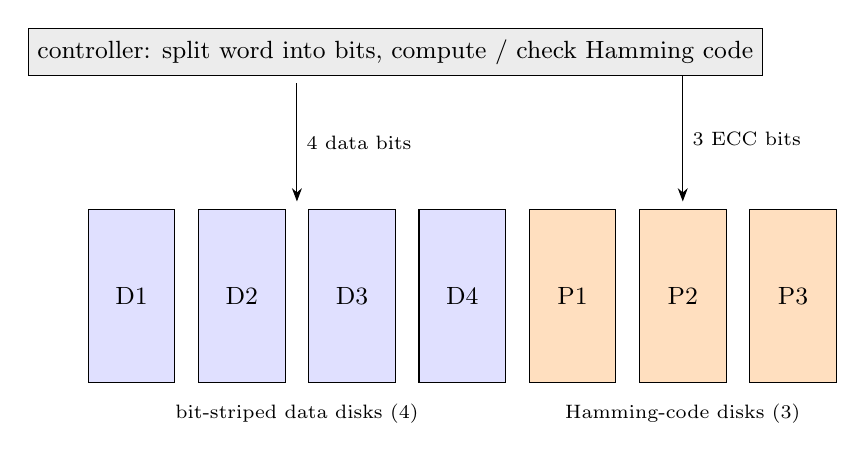
\begin{tikzpicture}[>=Stealth,font=\small]
\foreach \i/\l/\c in {0/{D1}/blue!12,1/{D2}/blue!12,2/{D3}/blue!12,3/{D4}/blue!12,4/{P1}/orange!25,5/{P2}/orange!25,6/{P3}/orange!25}
 { \draw[fill=\c] (\i*1.4,0) rectangle (\i*1.4+1.1,2.2); \node at (\i*1.4+0.55,1.1) {\l}; }
\node[font=\scriptsize] at (0.55+1.4*1.5,-0.4) {bit-striped data disks (4)};
\node[font=\scriptsize] at (0.55+1.4*5,-0.4) {Hamming-code disks (3)};
\draw[->] (0.55+1.4*1.5,3.8) -- (0.55+1.4*1.5,2.3) node[midway,right,font=\scriptsize]{4 data bits};
\node[draw,fill=gray!15,minimum width=7cm,minimum height=0.6cm,font=\small] at (3.9,4.2) {controller: split word into bits, compute / check Hamming code};
\draw[->] (0.55+1.4*5,3.9) -- (0.55+1.4*5,2.3) node[midway,right,font=\scriptsize]{3 ECC bits};
\end{tikzpicture}
\end{document}
